\chapter{Umsetzung\label{chap3:Drittes-Kapitel}}

Nachfolgend wird ein Konzept vorgestellt, mit welchem es möglich ist E-MES auf ungenutzten Code hin zu untersuchen. Um solchen Code zu identifizieren, wird eine dynamische Codeanalyse eingesetzt. Das dazu benötigte Konzept wird in \autoref{sec3.1:Unterpunkt-1} erläutert und die dazugehörige Implementierung wird in \autoref{sec3.2:Unterpunkt-2} aufgezeigt.


\section{Konzept\label{sec3.1:Unterpunkt-1}}

Eine Möglichkeit um ungenutzten Code innerhalb von E-MES zu identifizieren, wäre es die Aufrufhäufigkeit von Klassen und Methoden zu überwachen, indem man vor der Ausführung des Codes in jede Methode einen Zähler implementiert, welcher beim Aufruf hochgezählt wird. Dies würde jedoch einen hohen Implementierungsaufwand und eine permanente Änderung der Codebasis zur Folge haben.

Ein anderer Ansatz beruht auf der Manipulation des, zur Laufzeit zur Verfügung stehenden Bytecodes. Solch eine Manipulation ist mithilfe von Java-Agenten und der Klassenbibliothek Javassist realisierbar.

Java-Agenten bestehen aus speziellen Klassen, welche in der Lage sind eine laufende Java-Instanz innerhalb einer JVM \glqq abzufangen\grqq{} und deren Bytecode mithilfe von Javassist zu untersuchen und zu ändern. Man unterscheidet die Java-Agenten in statische und dynamische Agenten. Bei den statischen Agenten, wird die Manipulation des Bytecodes kurz vor der Ausführung der Codebasis durchgeführt (Bevor die Klassen von der JVM geladen werden). Bei dynamischen Agenten hingegen, ist eine Manipulation des Bytecodes auch während der Laufzeit möglich (Nachdem die Klassen von der JVM bereits geladen wurden). \cite{ManojDebnath.2020}

Das innerhalb dieser Praxisarbeit entworfene Konzept besteht nun daraus, einen dynamischen Java-Agent während der Laufzeit von E-MES auszuführen und eine Manipulation des Bytecodes zu erzeugen, um so jeden Methodenaufruf im System zu überwachen.

\section{Implementierung\label{sec3.2:Unterpunkt-2}}

Wie bereits geschildert besteht die Implementierung für die Überwachung der Methodenaufrufe aus einem dynamischen Java-Agenten, welcher mithilfe von Javassist den Bytecode von E-MES während der Laufzeit manipuliert.

Es sind drei unabhängige Programme entstanden:
\begin{description}
    \item[EMESAgentAttacher:]\hfill \\
    Dem \glqq Attacher\grqq{} wird die jeweilige Prozess-ID oder der Prozessname, des zu manipulierenden Programms, als Parameter übergeben. Mithilfe von diesem Parameter wird die dazugehörige virtuelle Maschine gesucht und das Programm \glqq EMESDynamicAgent\grqq{} hinzu geladen.
    \item[EMESDynamicAgent:]\hfill \\
    Dieses Programm stellt den eigentlichen Java-Agenten dar. Ziel ist es, die Manipulation nach dem Start, also während der Laufzeit von E-MES, durchzuführen. Deshalb wurde ein dynamischer Agent implementiert. Dessen Einsprungsmethode ist die agentmain-Methode:
    \begin{lstlisting}
    public static void agentmain(String agentArgs, Instrumentation inst){
        ...
    }
    \end{lstlisting}
    Mithilfe des übergebenen Parameters \glqq inst\grqq{} erhält der Java-Agent alle geladenen Klassen. Gefiltert nach den Packages der Klassen wird nun entschieden, welche Klassen manipuliert werden sollen und welche nicht.

    Wurde eine Klasse ausgesucht, werden nun alle Methoden dieser Klasse mithilfe von Javassist manipuliert. Hierfür werden die folgenden Codezeilen vom Agenten ausgeführt, welche dafür sorgen, dass am Anfang jeder manipulierten Methode ein Aufruf zu einer Java-Bean erfolgt.
    \begin{lstlisting}
    StringBuilder insertString = new StringBuilder();
    insertString.append("InitialContext context = new InitialContext();");
    insertString.append("CountCollector collector = (CountCollector) context.lookup(CountCollector.LOOKUP);");
    insertString.append("collector.notifyStats(\""+className+"\", \""+methodName+"\");");
    method.insertBefore(insertString.toString());
    \end{lstlisting}
    In diesem Fall ist die Java-Bean die Klasse \glqq CountCollector\grqq{} und wird über einen LOOKUP-String im Context gefunden.
    \item[addon-methodCounter:]\hfill \\
    Jede nun manipulierte Methode von E-MES ruft am Anfang ihrer Prozedur die Java-Bean auf. Übergeben werden der Klassen- und Methodenname. Die Bean überprüft anhand einer Java-Map, ob die Klassen-Methoden-Kombination bereits vorhanden ist und ergänzt diese, falls sie nicht vorhanden ist. Andernfalls wird die Anzahl der Aufrufhäufigkeit in der Map erhöht.
\end{description}

E-MES läuft auf Basis des Anwendungsservers Wildfly. Jener nach Java EE Standard implementierte Anwendungsserver weißt jedoch eine andere ClassLoader-Architektur auf, wie zum Beispiel die klassische ClassLoader-Architektur von Java. Üblicherweiße werden Java-Klassen zur Laufzeit von hierarchisch abhängigen ClassLoadern geladen. So genügt es den Java-Agenten mithilfe des \glqq Attachers\grqq{} an die laufende JVM anzubinden, um vollen Zugriff auf die geladenen Klassen zu erhalten.

\begin{figure}[h]
    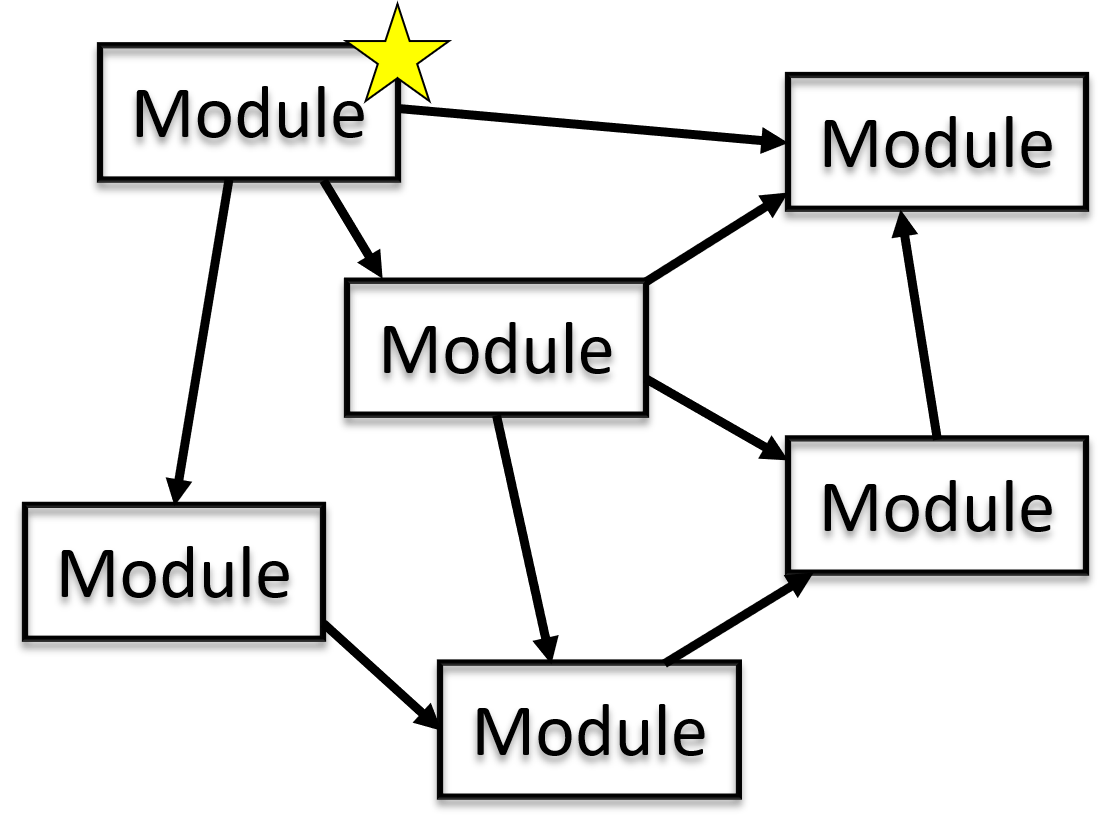
\includegraphics[width=0.5\linewidth]{images/Modules.png}
    \centering
    \caption{ClassLoader-Architektur von Wildfly}
    \label{fig:wildflyModules}
\end{figure}

Die ClassLoader-Architektur von Wildfly ist jedoch modular aufgebaut. Dies hat zur Folge, dass der Java-Agent einem Wildfly-Modul hinzugefügt werden muss, welches standartmäßig geladen wird und als Abhängigkeit von allen anderen Modulen dient. In Abbildung \ref{fig:wildflyModules} ist eine solche modulare ClassLoader-Architektur abgebildet. Beispielhaft dient hier das Modul oben links (mit Stern markiert) als \glqq Wurzel-Modul\grqq{}. Für die Implementierung eines Java-Agenten in E-MES wurde hierfür das Modul \glqq org.jboss.vfs\grqq{} ausgesucht, da es für das \glqq Virtual File System\grqq{} innerhalb von Wildfly zuständig ist und daher als Abhängigkeit für andere Module dient.